\documentclass[conference]{IEEEtran}
\IEEEoverridecommandlockouts
\usepackage{cite}
\usepackage{amsmath,amssymb,amsfonts}
\usepackage{mathtools}
\usepackage{booktabs}
\usepackage{enumitem}
\usepackage{tikz}
\usetikzlibrary{arrows.meta,positioning}

\newcommand{\sat}{\operatorname{sat}}
\newcommand{\diag}{\operatorname{diag}}

\begin{document}

\title{Quanser 3-DOF Gyroscope:\\ Hardware Physics, Identification, Modelling, and the Complete Controller Suite\\
{\footnotesize Mathematical foundations for offline simulation, digital-twin, and hardware execution}}

\author{\IEEEauthorblockN{Gandhi Contreras}
\IEEEauthorblockA{\textit{Electrical and Computer Engineering}, New Mexico State University, Las Cruces, NM, USA \\ gandhico@nmsu.edu}}

\maketitle

\begin{abstract}
The 3-DOF gyroscope is a high-speed flywheel carried in a gimbal train, the laboratory embodiment of angular-momentum physics: gimbal torques are transmitted across axes through gyroscopic coupling rather than direct actuation. This paper develops the device end to end: the power and slip-ring electrical path, the rotor and gimbal motor electromechanics, the angular-momentum dynamics by the Newton--Euler formalism with the momentum-exchange interpretation, gimbal-lock geometry, encoder-based sensing, identification of inertias and friction, linearization about the spin operating point, and the complete controller suite --- PID, LQR, LQG, backstepping, sliding-mode, and NMPC --- for gimbal-angle command through gyroscopic torque.
\end{abstract}

\begin{IEEEkeywords}
Control-moment gyroscope, gimbal dynamics, angular momentum, gyroscopic coupling, LQR, LQG, backstepping, SMC, NMPC.
\end{IEEEkeywords}

%====================================================================
\section{Introduction}
A rotor (disc) spins at high rate $\Omega$ inside an inner (red) gimbal, itself carried by an outer (blue) gimbal on a base frame; DC motors torque the rotor spin axis and the gimbal axes, and encoders measure all angles. Let $\theta_r$ be the rotor spin angle, $\theta_i$ the inner-gimbal angle, and $\theta_o$ the outer-gimbal angle. The essential physics: with the rotor momentum $h = J_r\Omega$ large, torquing one gimbal produces motion of the \emph{other} through the gyroscopic moment $h\,\dot\theta\,\cos(\cdot)$ --- the control-moment-gyroscope (CMG) principle used in spacecraft attitude control, which this device isolates.

%====================================================================
\section{Hardware Physics}

\begin{figure*}[!t]
\centering
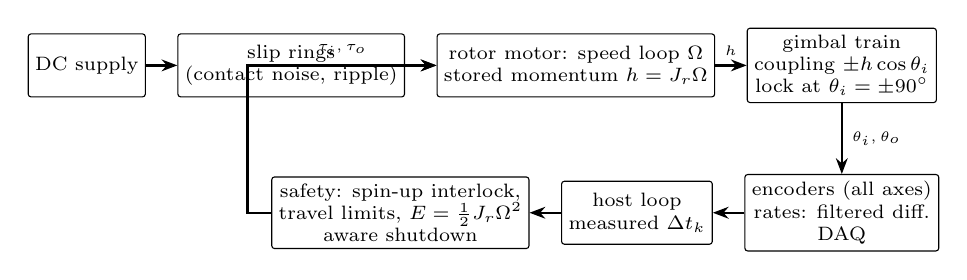
\begin{tikzpicture}[
  node distance=3mm and 4mm,
  blk/.style={draw, rounded corners=1pt, align=center, font=\scriptsize, inner sep=2.5pt, minimum height=8mm},
  lbl/.style={font=\tiny, align=center},
  arr/.style={-{Stealth[length=2mm]}, thick}
]

\node[blk] (sup) {DC supply};
\node[blk, right=of sup] (slip) {slip rings\\ (contact noise, ripple)};
\node[blk, right=of slip] (rotm) {rotor motor: speed loop $\Omega$\\ stored momentum $h = J_r\Omega$};
\node[blk, right=of rotm] (gim) {gimbal train\\ coupling $\pm h\cos\theta_i$\\ lock at $\theta_i = \pm90^\circ$};
\node[blk, below=9mm of gim] (enc) {encoders (all axes)\\ rates: filtered diff.\\ DAQ};
\node[blk, left=of enc] (loop) {host loop\\ measured $\Delta t_k$};
\node[blk, left=of loop] (safe) {safety: spin-up interlock,\\ travel limits, $E = \tfrac12 J_r\Omega^2$\\ aware shutdown};
\draw[arr] (sup) -- (slip);
\draw[arr] (slip) -- (rotm);
\draw[arr] (rotm) -- node[lbl, above] {$h$} (gim);
\draw[arr] (gim) -- node[lbl, right] {$\theta_i,\theta_o$} (enc);
\draw[arr] (enc) -- (loop);
\draw[arr] (loop) -- (safe);
\draw[arr] (safe.west) -- ++(-3mm,0) |- node[lbl, pos=0.75, above] {$\tau_i,\tau_o$} (rotm.west);
\end{tikzpicture}
\caption{3-DOF gyroscope signal chain: stored rotor momentum couples the gimbal axes; slip rings carry power and signal to the rotating assembly; spin-up interlocks govern the safety state machine.}
\label{fig:chain}
\end{figure*}
\subsection{Power path and slip rings}
The base supplies the gimbal motors directly; power and signals to the rotating inner assembly pass through \emph{slip rings} --- sliding contacts whose physics (contact resistance variation, brush noise) add measurement noise and a small torque ripple, and whose current rating bounds the rotor motor drive. PWM H-bridges drive each brushed DC motor with averaged terminal voltage $v = DV_s$, $|v|\le V_{\max}$.

\subsection{Motors and rotor spin loop}
Each motor: $L_a\dot i + R_m i + k_e\omega = v$, $\tau = k_t i$, electrical pole fast at the loop rate. The rotor axis runs a dedicated speed loop holding $\Omega$ constant; its physics matter to control only through the stored momentum $h = J_r\Omega$ and its regulation stiffness (a droop in $\Omega$ under gimbal maneuvers is a gain disturbance to every gyroscopic term). Spin-up obeys $J_r\dot\Omega = k_t i - b_r\Omega$, a first-order lag with minutes-scale thermal limits at high $\Omega$.

\subsection{Sensing, loop, and safety}
Quadrature encoders on all axes with resolutions $2\pi/N_k$; rates by filtered differentiation (measured-$\Delta t$ discipline as on all our platforms); rotor speed from its encoder frequency. Safety envelope: rotor spin-up interlock (gimbals locked or centred during spin-up), gimbal travel limits (hard stops + software), kinetic-energy awareness ($E = \tfrac12 J_r\Omega^2$ is large --- guards and controlled spin-down), current/thermal limits, watchdog with all-channel zero on fault.

%====================================================================
\section{Dynamics}
\subsection{Frames and angular velocities}
Base $\to$ outer gimbal (rotation $\theta_o$ about the base vertical $k$-axis) $\to$ inner gimbal (rotation $\theta_i$ about the outer gimbal's horizontal axis) $\to$ rotor (spin $\Omega$ about the inner gimbal's normal axis). Expressed in the inner-gimbal frame $(x_i, y_i, z_i)$ with spin about $z_i$:
\begin{equation}
\omega_i = \begin{bmatrix}
\dot\theta_o\cos\theta_i\\ \dot\theta_i\\ \dot\theta_o\sin\theta_i
\end{bmatrix},\qquad
\omega_{\mathrm{rotor}} = \omega_i + \Omega\, e_{z_i}.
\end{equation}

\subsection{Momentum-exchange equations}
With rotor inertia $J_r$ about spin and $J_t$ transverse, inner-gimbal inertia diag$(A_i, B_i, C_i)$, and outer-gimbal inertia $C_o$ about the base axis, Euler's equation $\dot H = \tau$ applied to the train yields, for the two controlled gimbal axes (spin regulated separately),
\begin{align}
&\bigl(B_i + J_t\bigr)\ddot\theta_i
+ \underbrace{h\,\dot\theta_o\cos\theta_i}_{\text{gyroscopic}}
+ \tfrac12\bigl(\Delta J\bigr)\dot\theta_o^2\sin2\theta_i
+ b_i\dot\theta_i = \tau_i,
\label{eq:inner}\\[2pt]
&J_o(\theta_i)\,\ddot\theta_o
- \underbrace{h\,\dot\theta_i\cos\theta_i}_{\text{gyroscopic}}
+ \Delta J\,\dot\theta_i\dot\theta_o\sin2\theta_i
+ b_o\dot\theta_o = \tau_o,
\label{eq:outer}
\end{align}
where $h = J_r\Omega$, $\Delta J$ collects the transverse-inertia asymmetries, and
$J_o(\theta_i) = C_o + A_i\sin^2\theta_i + (C_i + J_t)\cos^2\theta_i$ is the $\theta_i$-dependent outer-axis inertia. The physics to internalize: the dominant cross terms $\pm h\cos\theta_i\,\dot\theta$ are \emph{skew-symmetric} (they exchange momentum between axes without doing net work) and scale with the stored momentum --- torque one axis, and it is chiefly the \emph{other} axis that moves.

\subsection{Gimbal lock and operating point}
At $\theta_i = \pm90^\circ$ the projection $\cos\theta_i$ vanishes: the gyroscopic channel closes and outer-axis authority through the rotor disappears --- the gimbal-lock geometry. The nominal operating point is $\theta_i = 0$ with $\Omega$ constant; there the linearization of \eqref{eq:inner}--\eqref{eq:outer} is
\begin{equation}
\begin{aligned}
I_1\ddot\theta_i + b_i\dot\theta_i + h\,\dot\theta_o &= \tau_i,\\
I_2\ddot\theta_o + b_o\dot\theta_o - h\,\dot\theta_i &= \tau_o,
\end{aligned}
\label{eq:gyrolin}
\end{equation}
$I_1 = B_i + J_t$, $I_2 = J_o(0)$: a pair of damped integrators coupled by the skew gyroscopic matrix $\begin{bsmallmatrix}0 & h\\ -h & 0\end{bsmallmatrix}$. In state form $x = [\theta_i,\ \theta_o,\ \dot\theta_i,\ \dot\theta_o]^{\!\top}$, $u = [\tau_i,\ \tau_o]^{\!\top}$, the pair $(A,B)$ is controllable for $h\neq0$ \emph{even with one motor disabled} --- single-gimbal CMG control of the other axis, the canonical demonstration of this device.

%====================================================================
\section{Identification}

\begin{figure}[!t]
\centering
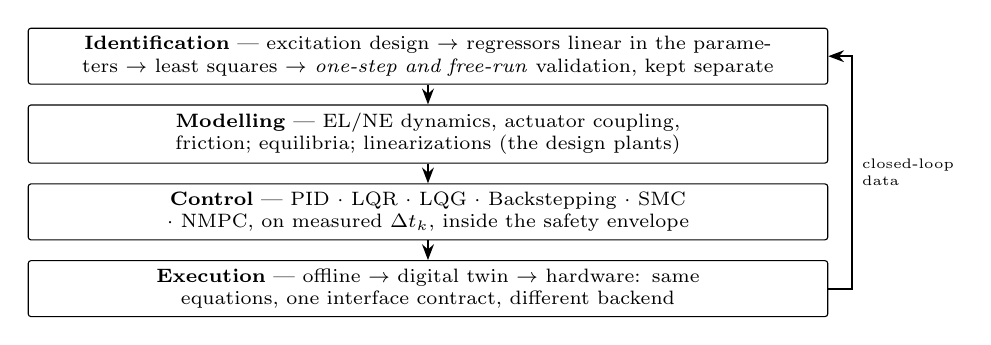
\begin{tikzpicture}[
  node distance=2.5mm,
  blk/.style={draw, rounded corners=1pt, align=center, font=\scriptsize, inner sep=3pt, text width=0.82\columnwidth},
  arr/.style={-{Stealth[length=2mm]}, thick}
]
\node[blk] (id) {\textbf{Identification} --- excitation design $\to$ regressors linear in the parameters $\to$ least squares $\to$ \emph{one-step and free-run} validation, kept separate};
\node[blk, below=of id] (mod) {\textbf{Modelling} --- EL/NE dynamics, actuator coupling, friction; equilibria; linearizations (the design plants)};
\node[blk, below=of mod] (ctl) {\textbf{Control} --- PID $\cdot$ LQR $\cdot$ LQG $\cdot$ Backstepping $\cdot$ SMC $\cdot$ NMPC, on measured $\Delta t_k$, inside the safety envelope};
\node[blk, below=of ctl] (exe) {\textbf{Execution} --- offline $\to$ digital twin $\to$ hardware: same equations, one interface contract, different backend};
\draw[arr] (id) -- (mod);
\draw[arr] (mod) -- (ctl);
\draw[arr] (ctl) -- (exe);
\draw[arr] (exe.east) -- ++(3mm,0) |- node[font=\tiny, pos=0.25, right, align=left] {closed-loop\\ data} (id.east);
\end{tikzpicture}
\caption{The workflow every platform in this series follows: identification feeds modelling, modelling feeds the controller suite, and all stages run unchanged across the three execution targets; closed-loop records return to identification.}
\label{fig:workflow}
\end{figure}
E1) \emph{rotor}: spin-up/coast-down first-order responses fit $J_r/b_r$ and $k_t/R_m$; $h$ then follows from measured $\Omega$. E2) \emph{gimbal inertias and friction}: with $\Omega = 0$ the axes decouple to $I\ddot\theta + b\dot\theta + \tau_c\tanh(\dot\theta/\epsilon) = \tau$; steps and chirps give $(I_1, I_2, b_i, b_o, \tau_c)$ by least squares (linear in the parameters with filtered $\ddot\theta$). E3) \emph{gyroscopic gain}: with $\Omega$ at operating speed, torque one axis with a doublet and regress the \emph{other} axis's response against $h\cos\theta_i\,\dot\theta$; consistency of $\hat h$ with $J_r\Omega$ from E1 is the model-validation gate. E4) black-box MIMO ARX cross-check on \eqref{eq:gyrolin}; one-step and free-run reported separately.

%====================================================================
\section{Control Suite}
All laws command $u = [\tau_i, \tau_o]^{\!\top}$ through the motor gains, clip at the drive limits, and use filtered rates with measured $\Delta t_k$. The plant \eqref{eq:gyrolin} is genuinely two-input two-output with skew coupling: decentralized designs must treat the coupling as disturbance, centralized designs exploit it.

\subsection{PID}
Per-axis PD/PID on $(\theta_i, \theta_o)$ treating the gyroscopic cross term as a disturbance --- adequate at low $h$, degrading as $h$ grows (the coupling scales with $\Omega$ while the plant poles do not): the physically transparent motivation for model-based design. Decoupling feedforward $\tau_i^{\mathrm{ff}} = h\dot\theta_o\cos\theta_i$, $\tau_o^{\mathrm{ff}} = -h\dot\theta_i\cos\theta_i$ cancels the coupling exactly at the identified $\hat h$ and turns PID into two independent loops --- the cheapest high-value model injection on this device.

\subsection{LQR / LQG}
$u = -K_{\mathrm{lqr}}(x - x_r)$, CARE on \eqref{eq:gyrolin} with Bryson-scaled $Q, R$; the optimal gain automatically contains the cross-feed structure (nonzero off-diagonal entries proportional to $h$). LQG closes from encoders alone: Kalman--Bucy filter with measurement covariance from encoder quantization, process covariance absorbing friction error; estimator propagated with measured $\Delta t_k$; separation nominal.

\subsection{Backstepping}
The cascade $\theta \to \dot\theta \to \tau$ is strict feedback per axis with the coupling entering the second stage: $z_1 = \theta - \theta_r$, virtual rate $\dot\theta^d = \dot\theta_r - c_1 z_1$, $z_2 = \dot\theta - \dot\theta^d$, and
\begin{equation}
\tau = \hat b\,\dot\theta \pm \hat h\cos\theta_i\,\dot\theta_{\mathrm{other}} + I\bigl(\ddot\theta^d - z_1 - c_2 z_2\bigr),
\end{equation}
i.e., exact cancellation of the identified coupling inside the Lyapunov design $V = \tfrac12\sum(z_1^2 + z_2^2)$, $\dot V = -\sum c_i z_i^2 + \tilde h(\cdot)$, with the residual bounded by the identification error $\tilde h$ --- the quantitative link between E3 accuracy and achievable gains.

\subsection{Sliding mode}
Per-axis surfaces $s = \dot e + \lambda e$; equivalent control from \eqref{eq:gyrolin} including the cross term; switching gain $\eta$ sized to the \emph{unmatched-looking but actually matched} uncertainty $|\tilde h||\dot\theta_{\mathrm{other}}|_{\max}$ plus friction error; boundary layer $\phi$ above the differentiated-encoder noise floor. Reaching condition $\tfrac{d}{dt}\tfrac12 s^2 \le -(\eta - \bar\rho)|s|$ as on our other platforms.

\subsection{NMPC}
Receding horizon on the full nonlinear \eqref{eq:inner}--\eqref{eq:outer} (RK4), cost $\sum \|x_k - x_r\|_Q^2 + \|u_k\|_R^2 + V_f$ with LQR terminal weight, constraints: torque limits, gimbal travel limits, and --- the constraint unique to this device --- a \emph{gimbal-lock avoidance} bound $|\theta_i| \le \bar\theta_i < 90^\circ$ keeping the gyroscopic channel open; NMPC is the natural home for that geometric constraint, which no unconstrained law respects. Real-time reductions as on our other platforms (short horizon, move blocking, warm start).

%====================================================================
\section{Execution Modes and Conclusion}
Offline: \eqref{eq:inner}--\eqref{eq:outer} with encoder quantization, slip-ring noise, and $\Omega$-droop models injectable; digital twin under the same command/measurement contract; hardware under the spin-up interlocks and travel limits. The device delivers the purest laboratory form of momentum-exchange control: skew gyroscopic coupling proportional to stored momentum, a $\cos\theta_i$ authority geometry with its lock singularity, parameter-linear identification with a physical consistency gate ($\hat h$ vs.\ $J_r\Omega$), and the six-controller suite in which model knowledge buys exactly what the physics says it should --- cancellation or exploitation of the cross-axis momentum flow.

\bibliographystyle{IEEEtran}
\begin{thebibliography}{9}
\bibitem{wie2008} B.~Wie, \emph{Space Vehicle Dynamics and Control}, 2nd ed. AIAA, 2008.
\bibitem{greenwood1988} D.~T. Greenwood, \emph{Principles of Dynamics}, 2nd ed. Prentice Hall, 1988.
\bibitem{quanser_gyro} Quanser Consulting Inc., \emph{3 DOF Gyroscope User Manual}, Markham, ON, Canada.
\bibitem{khalil2002} H.~K. Khalil, \emph{Nonlinear Systems}, 3rd ed. Prentice Hall, 2002.
\bibitem{krstic1995} M.~Krsti\'c, I.~Kanellakopoulos, and P.~Kokotovi\'c, \emph{Nonlinear and Adaptive Control Design}. Wiley, 1995.
\bibitem{utkin1992} V.~Utkin, \emph{Sliding Modes in Control and Optimization}. Springer, 1992.
\bibitem{rawlings2017} J.~B. Rawlings, D.~Q. Mayne, and M.~Diehl, \emph{Model Predictive Control}, 2nd ed. Nob Hill, 2017.
\bibitem{ljung1999} L.~Ljung, \emph{System Identification: Theory for the User}, 2nd ed. Prentice Hall, 1999.
\end{thebibliography}

\end{document}
